\documentclass[11 pt, a4paper]{article}
\usepackage[left=1.5cm,top= 1.5cm,right= 1.5cm,bottom=1.5cm]{geometry}
\usepackage[spanish]{babel}
\usepackage{amsthm}
\usepackage{graphicx}
\theoremstyle{definition}
\newtheorem{definicion}{Definici\'on}[section]
\graphicspath{{img/}}
\usepackage[utf8]{inputenc} 
\usepackage{amsmath,amssymb,amsfonts,latexsym} %Soporte para símbolos y font matemáticos
\usepackage{float}
\usepackage{amsthm}
\usepackage{enumerate}
% \usepackage[options]{algorithm2e}
\DeclareGraphicsExtensions{.pdf,.png,.jpg}
\DeclareGraphicsRule{.wmf}{bmp}{}{}
\newtheorem{no}{Nota}
\author{Trinidad Hern\'andez Norma Ver\'onica \\
        Vilchis Dom\'inguez Miguel Alonso}
\title{Tarea 2}
\date{}
\begin{document}
\maketitle

\section{Ejercicios}

\begin{enumerate}
 \item \textbf{Demostrar si las siguientes funciones son $\theta(n^2)$}
 \no Sea $f(n)$ una función por definición si $f(n) \in \theta(g(n))$ 
 implica que $ \exists c_1, c_2 \in \mathbb{N} $ y $\exists n_0 \in \mathbb{N}$ 
 tales que $0 \leq c_1*g(n) \leq f(n) \leq c_2*g(n)$.
 \begin{enumerate}
  \item $60n^2 + 5n +1$\\
  Por demostrar que $60n^2 + 5n +1 \in \theta(n^2)$. Por la \textbf{Nota 1}
  implica mostrar las constantes tales que la función queda acotada por 
  $n^2$ al multiplicarla por dichas constantes. Es decir:\\
  \begin{equation} 
   c_1* n^2 \leq 60n^2 + 5n +1 \leq c_2 * n^2 
   \end{equation}
  Sii
  \[ c_1 \leq 60 + \frac{5}{n} + \frac{1}{n^2} \leq c_2 \]
  Se propone $n_0 = 10$, $c_1 = 59$, $c_2 = 70$  Por lo que
  \[ 59 \leq 60 + \frac{5}{10} + \frac{1}{100} = \frac{6051}{100} \leq 70  \]
  Con lo que se sigue cumpliendo la desigualdad. Para finalizar la demostración 
  basta con mostrar que la desigualdad se sigue cumpliendo para
  $n > n_0$ con $n \in \mathbb{N}$.\\ 
  En efecto, para hacer una buena aproximación de lo que ocurre con 
  $n$ grandes, tomamos el $lim_{n \rightarrow \infty}$. Es decir:
  \[ lim_{n \rightarrow \infty} \left(60 + \frac{5}{n} + \frac{1}{n^2} \right)\]
   \[  = lim_{n \rightarrow \infty} 60 + lim_{n \rightarrow \infty} \frac{5}{n} + lim_{n \rightarrow \infty} \frac{1}{n^2} \]
  \[  = 60 + 0+0 \]
  Con lo que, se sigue cumpliendo la desigualdad $(1)$
  \begin{figure}[H]
         \centering
          %trim left bottom right top
          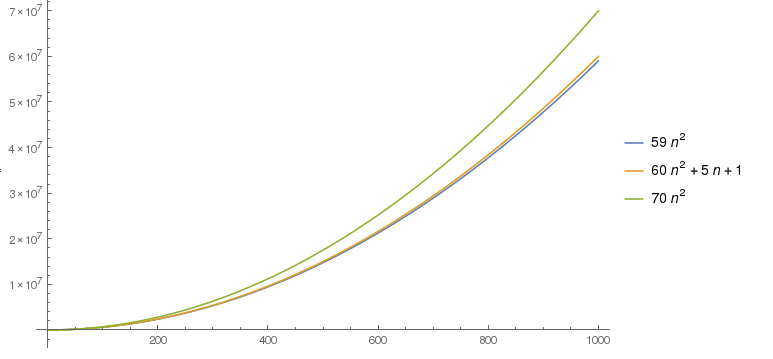
\includegraphics[trim=0cm 0cm 0cm 0cm, width=15cm]{inciso1.png} 
          \caption{Gráfica que muestra la comparación entre las funciones}
      \end{figure}
  \item $2n^2 - 16 n + 35$\\
  Siguendo un procedimiento parecido al inciso a, lo que haremos 
  para mostrar que $2n^2 - 16 n + 35 \in \theta(n^2)$ será utilizar 
  la definición que se dio en la \textbf{Nota 1}, por lo que:
  \begin{equation}
   c_1*n^2 \leq 2n^2 - 16 n + 35 \leq c_2*n^2
  \end{equation}
  Sii
  \[c_1 \leq 2 - \frac{16}{n} + \frac{35}{n^2} \leq c_2 \]
  Se propone $n_0 = 16$, $c_1 = 1$ y $c_2 = 3$ obteniendo:
  
  \[ 1 \leq 2 - \frac{16}{10} + \frac{35}{256} = \frac{281}{256}\leq 3 \]
  Tomando el límite cuando $n$ tiende a infinito, para mostrar que la 
  desigualdad se cumple para  $n_0 < n \in \mathbb{N}$
  \[
   lim_{n \rightarrow \infty} \left( 2 - \frac{16}{n} + \frac{35}{n^2}\right)\]
   \[= lim_{n \rightarrow \infty} 2 - lim_{n \rightarrow \infty} \frac{16}{n} + lim_{n \rightarrow \infty} \frac{35}{n^2}\]
   \[= 2 - 0 +0   \]
  Con lo que se conserva la desigualdad $(2)$
    \begin{figure}[H]
         \centering
          %trim left bottom right top
          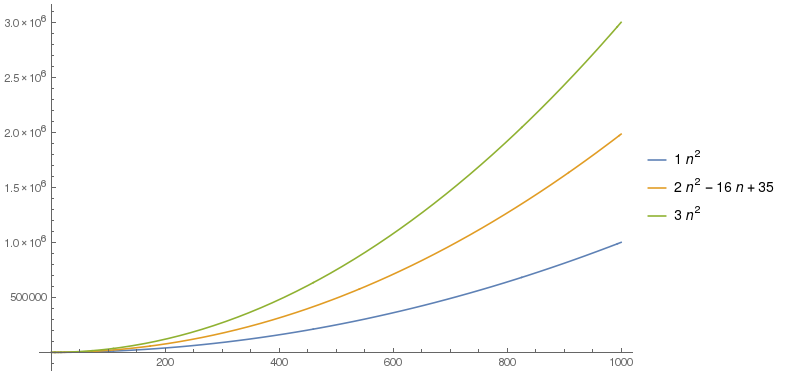
\includegraphics[trim=0cm 0cm 0cm 0cm, width=15cm]{inciso2.png} 
          \caption{Gráfica que muestra la comparación entre las funciones}
      \end{figure}
   \item $3 n^2 + 2* n\ ln\ n$
  Por demostrar que $3 n^2 + 2* n\ ln\ n \in \theta (n^2) $, en efecto:
  \begin{equation}
      c_1*n^2 \leq 3 n^2 + 2 * n\ ln\ n\leq c_2*n^2
  \end{equation}
  Sii
  \[  c_1\leq 3 + \frac{2 * \ ln\ n} {n}\leq c_2\]
  Si proponemos $n_0 = 128$, $c_1= 2$ y $c_2 = 4 $ obtenemos:
  \[ 2 \leq  3 + \frac{2 * \ ln\ 128} {128} = 3 + \frac{7}{64}= \frac{199}{64} \leq 4 \]
 Para demostrar que la desigualdad $(3)$ se cumple para $n_0 < n \in \mathbb{N}$
 tomamos $lim_{n \rightarrow \infty}$: 
 \[lim_{n \rightarrow \infty} \left(3 + \frac{2 * \ ln\ n} {n}\right)\]
  \[= 3 +  lim_{n \rightarrow \infty} \frac{2 * \ ln\ n} {n}\]
 \[ = 3 +0 \]
 Con lo que la desigualdad $(3)$ se conserva.
   \begin{figure}[H]
         \centering
          %trim left bottom right top
          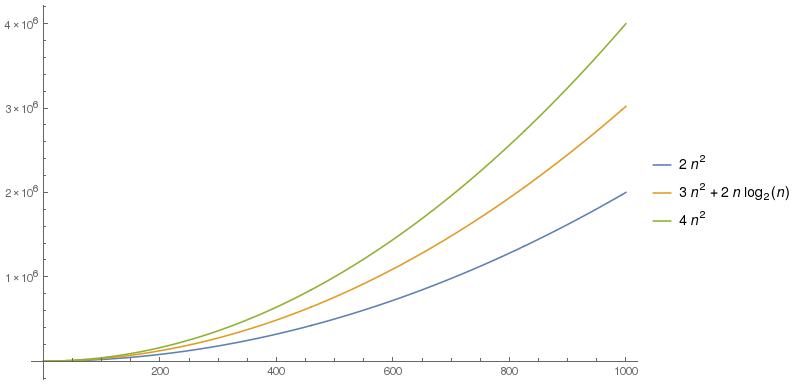
\includegraphics[trim=0cm 0cm 0cm 0cm, width=15cm]{inciso3.png} 
          \caption{Gráfica que muestra la comparación entre las funciones}
      \end{figure}



  
  
  \item $2+4+6+ ... + 2m$
  Si hacemos $n = \frac{m}{2}$ entonces podemos expresar la suma de la siguiente manera
  $2*(1+2+...+ n)$, lo cual es la suma de los primeros $n$ naturales, con lo que queda 
  representado por 
  \[2*\left( \frac{(n)*(n+1)}{2}\right) = n^2 + n \]
  Por lo que el problema se reduce a demostrar que $n^2 +n \in \theta(n^2)$, es 
  decir: 
  \begin{equation}
      c_1*n^2 \leq n^2 + n\leq c_2*n^2
  \end{equation}
  Sii 
  \[  c_1 \leq 1 + \frac{1}{n}\leq c_2 \]
  Si tomamos $n_0 = 10$, $c_1 = 1$ y $c_2 = 2$ con lo que: 
  \[ 
    1 \leq 1 + \frac{1}{10} = \frac{11}{10} \leq 2
  \]
  
  Tomando el límite cuando $n$ tiende a infinito, para demostrar que 
  la desigualdad se sigue cumpliendo para $n_0 < n \in \mathbb{N}$
  
    \[
   lim_{n \rightarrow \infty} 1 + \frac{1}{n} \]
   \[= lim_{n \rightarrow \infty} 1 + lim_{n \rightarrow \infty} \frac{1}{n} \]
   \[= 1+0   \]
  Con lo que la desigualdad $(4)$ se sigue conservando.  
 
   \begin{figure}[H]
         \centering
          %trim left bottom right top
          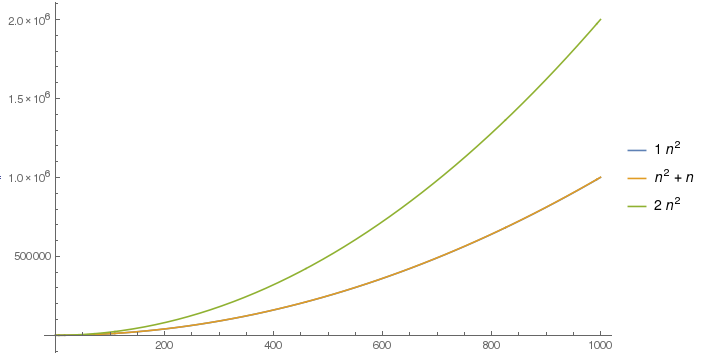
\includegraphics[trim=0cm 0cm 0cm 0cm, width=15cm]{inciso4.png} 
          \caption{Gráfica que muestra la comparación entre las funciones}
      \end{figure}
  \item $1.\ for\ i = 1 \ to \ n$\\
        $2.\ \ \ \ for\ j = 1\ to\ i$\\
        $3.\ \ \ \ \ \ \ \ for\ k = 1\ to\ i$ \\
        $4.\ \ \ \ \ \ \ \ \ \ \ \ x= x +1$ \\                     
El análisis de complejidad del código de arriba puede realizarse de la siguiente manera:
La línea 1 toma $c_1* n$ operaciones, que son los incrementos de i y la comparación booleana, para alguna 
constante $c_1$, más las asignación inicial la cual es despreciable 
debido a que se trata de una constante.\\
En la línea 2, la cantidad de operaciones que se van a realizar son
$\sum_{j = 1}^i c_2*j$ para alguna constante $c_2$, note que $c_2*\sum_{j = 1}^i j= c_2*\left(\frac{n*(n+1)}{2}\right)$\\
Para la línea 3, lo que tenemos es  $\sum_{k = 1}^{i} c_3*k^2$, para
alguna constante $c_3$,debido al for de la línea $2$ y al propio
for de la línea $3$, es decir, 
$c_3\sum_{k = 1}^{i} k^2 = c_3 * \left(\frac{n*(n+1)*(2n+1)}{6} \right)$\\
Básicamente para la línea 4, lo que tenemos es la misma complejidad 
que la línea 3, diferido por una constante. i.e.  $c_4 * \left(\frac{n*(n+1)*(2n+1)}{6} \right)$\\
Por lo que la complejidad del código es: 
\[c_1* n + c_2*\left(\frac{n*(n+1)}{2}\right) +c_3 * \left(\frac{n*(n+1)*(2n+1)}{6} \right) + c_4 * \left(\frac{n*(n+1)*(2n+1)}{6} \right) \]
Multiplicando por 12 y desarrollando obtenemos: 
\[c'_1* n + c'_2*\left(n^2 +n )\right) +c'_3 * \left(n + 3 n^2 + 2 n^3 \right) = c'_3*2n^3+ c'_2*n^2+ c'_1*n + c_0 *n\]
Basta notar que no se cumple $\theta(n^3) \notin \theta(n^2) $, supongamos que se cumple
implica que $n < c_n$ para alguna constante $c_n$, sin embargo siempre se puede dar una 
n mayor a la constante establecida, y 
si consideramos la \textbf{Nota 1}, implicaría que no podemos encontrar el $n_0 $ tal que 
$n_0 < n \in \mathbb{N}$ que cumpla con la proposición. \\

Por lo tanto, el código no se encuentra en el orden de $\theta(n^2)$
 \end{enumerate}
\item 2.- \textbf{Ordenar funciones por ordenamiento asintótico}\\
El orden que encontramos fue el siguiente: 
\[
2^{2^{n+1}} > 2^{2^{n}} > (n+1)! > n! > e^{n} > n2^n > 2^n > \left(\frac{3}{2} \right) > n^3\]
\[>  log (n^{log (n)}) = n^{log(log(n))} > 4^{log(n)} = n^2 > (log(n)) ! > n log(n)\]
\[ > log(n!) > 2^{log(n)} = n > log^2 (n) > \sqrt{2}^{log_2(n)} > 2^{\sqrt{2 log(n)}}\]
\[> log(n) > 2^{log^*(n)} > \sqrt{log_2(n)} > log^*(n) > ln(ln(n)) > log(log^*(n)) > n^{\frac{1}{log(n)}} = 1\]

El orden lo obtuvimos por medio de graficación, las gráficas son las siguientes: 
 \begin{figure}[H]
         \centering
          %trim left bottom right top
          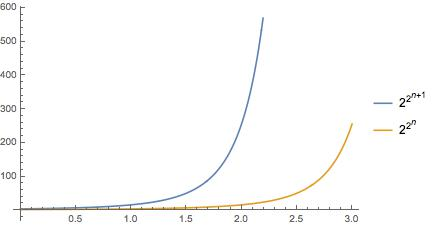
\includegraphics[trim=0cm 0cm 0cm 0cm, width=12cm]{1.jpg} 
      \end{figure}
 \begin{figure}[H]
         \centering
          %trim left bottom right top
          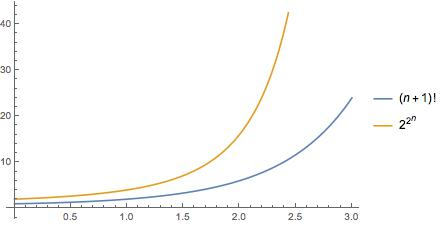
\includegraphics[trim=0cm 0cm 0cm 0cm, width=12cm]{2.jpg} 
      \end{figure} \begin{figure}[H]
         \centering
          %trim left bottom right top
          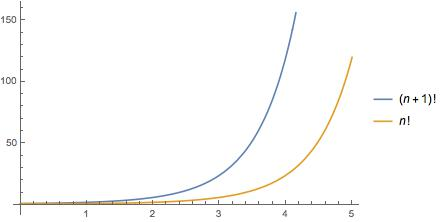
\includegraphics[trim=0cm 0cm 0cm 0cm, width=12cm]{3.jpg} 
      \end{figure} \begin{figure}[H]
         \centering
          %trim left bottom right top
          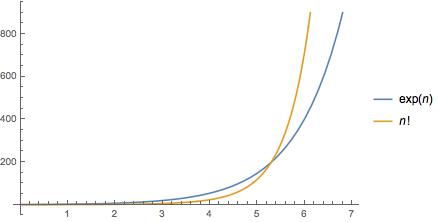
\includegraphics[trim=0cm 0cm 0cm 0cm, width=12cm]{4.jpg} 
      \end{figure} \begin{figure}[H]
         \centering
          %trim left bottom right top
          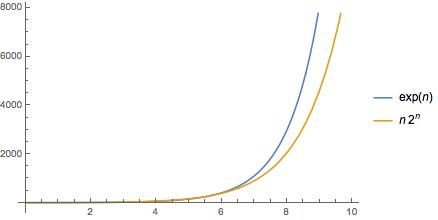
\includegraphics[trim=0cm 0cm 0cm 0cm, width=12cm]{5.jpg} 
      \end{figure} \begin{figure}[H]
         \centering
          %trim left bottom right top
          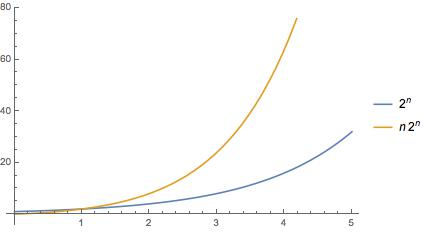
\includegraphics[trim=0cm 0cm 0cm 0cm, width=12cm]{6.jpg} 
      \end{figure} \begin{figure}[H]
         \centering
          %trim left bottom right top
          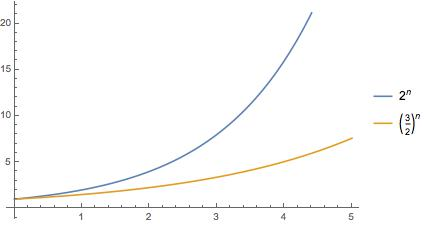
\includegraphics[trim=0cm 0cm 0cm 0cm, width=12cm]{7.jpg} 
      \end{figure} \begin{figure}[H]
         \centering
          %trim left bottom right top
          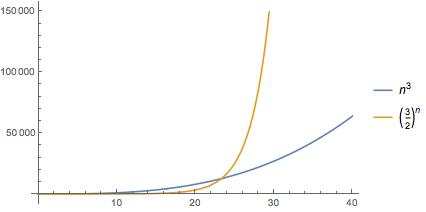
\includegraphics[trim=0cm 0cm 0cm 0cm, width=12cm]{8.jpg} 
      \end{figure} \begin{figure}[H]
         \centering
          %trim left bottom right top
          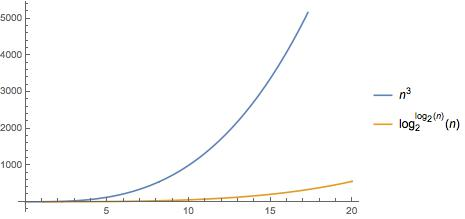
\includegraphics[trim=0cm 0cm 0cm 0cm, width=12cm]{9.jpg} 
      \end{figure} \begin{figure}[H]
         \centering
          %trim left bottom right top
          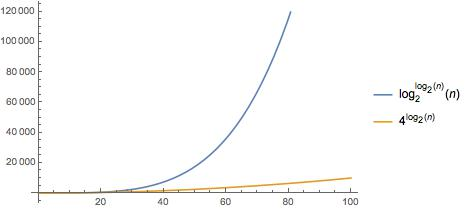
\includegraphics[trim=0cm 0cm 0cm 0cm, width=12cm]{10.jpg} 
      \end{figure} \begin{figure}[H]
         \centering
          %trim left bottom right top
          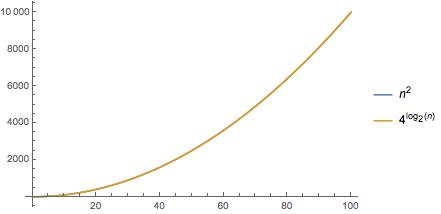
\includegraphics[trim=0cm 0cm 0cm 0cm, width=12cm]{11.jpg} 
      \end{figure} \begin{figure}[H]
         \centering
          %trim left bottom right top
          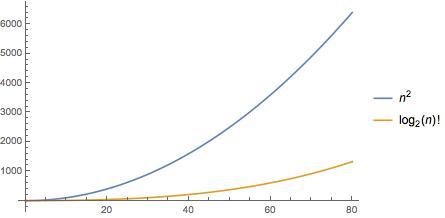
\includegraphics[trim=0cm 0cm 0cm 0cm, width=12cm]{12.jpg} 
      \end{figure} \begin{figure}[H]
         \centering
          %trim left bottom right top
          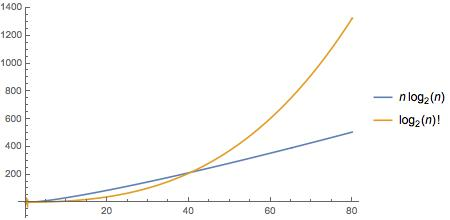
\includegraphics[trim=0cm 0cm 0cm 0cm, width=12cm]{13.jpg} 
      \end{figure} \begin{figure}[H]
         \centering
          %trim left bottom right top
          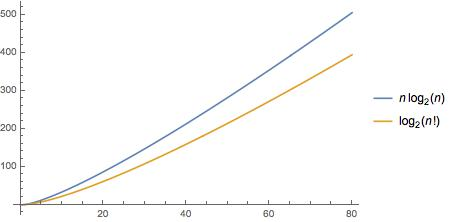
\includegraphics[trim=0cm 0cm 0cm 0cm, width=12cm]{14.jpg} 
      \end{figure} \begin{figure}[H]
         \centering
          %trim left bottom right top
          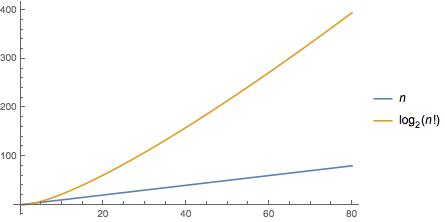
\includegraphics[trim=0cm 0cm 0cm 0cm, width=12cm]{15.jpg} 
      \end{figure} \begin{figure}[H]
         \centering
          %trim left bottom right top
          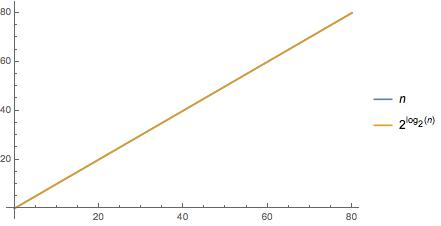
\includegraphics[trim=0cm 0cm 0cm 0cm, width=12cm]{16.jpg} 
      \end{figure} \begin{figure}[H]
         \centering
          %trim left bottom right top
          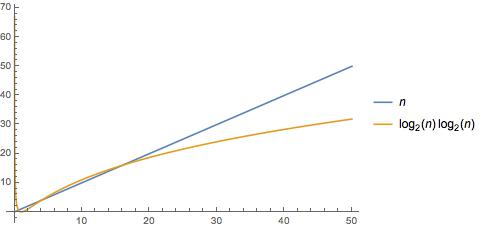
\includegraphics[trim=0cm 0cm 0cm 0cm, width=12cm]{17.jpg} 
      \end{figure} \begin{figure}[H]
         \centering
          %trim left bottom right top
          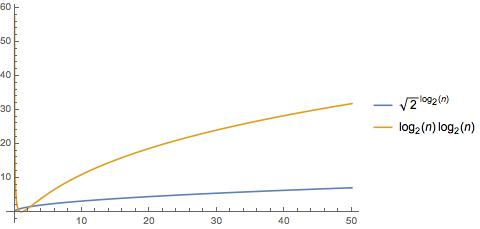
\includegraphics[trim=0cm 0cm 0cm 0cm, width=12cm]{18.jpg} 
      \end{figure} \begin{figure}[H]
         \centering
          %trim left bottom right top
          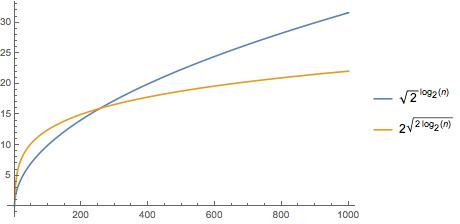
\includegraphics[trim=0cm 0cm 0cm 0cm, width=12cm]{19.jpg} 
      \end{figure} 
      Mostrando las gráficas en conjunto:
      \begin{figure}[H]
         \centering
          %trim left bottom right top
          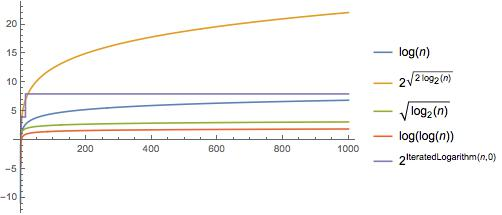
\includegraphics[trim=0cm 0cm 0cm 0cm, width=15cm]{todas.jpg} 
      \end{figure} \begin{figure}[H]
         \centering
          %trim left bottom right top
          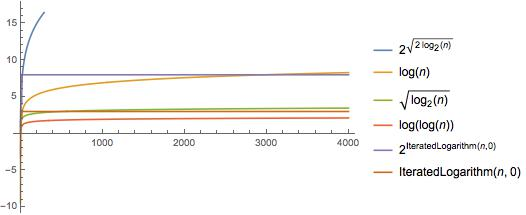
\includegraphics[trim=0cm 0cm 0cm 0cm, width=15cm]{todas2.jpg} 
      \end{figure} \begin{figure}[H]
         \centering
          %trim left bottom right top
          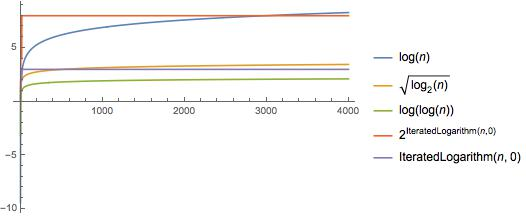
\includegraphics[trim=0cm 0cm 0cm 0cm, width=15cm]{todas3.jpg} 
      \end{figure} \begin{figure}[H]
         \centering
          %trim left bottom right top
          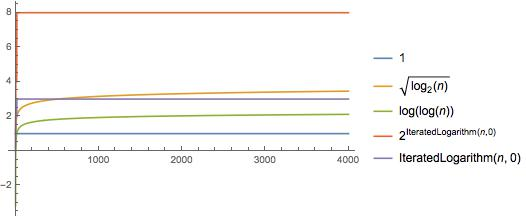
\includegraphics[trim=0cm 0cm 0cm 0cm, width=15cm]{todas4.jpg} 
      \end{figure}

\end{enumerate}
\end{document}

